%%%%%%%%%%%%%%%%%%%%%%%%
% DO NOT TOUCH THIS PART
\documentclass{hitec}
\newcommand{\HT}{\textsc{\raisebox{0.1em}{h}\raisebox{-0.1em}{i}%
	\raisebox{0.1em}{t}\raisebox{-0.1em}{e}\raisebox{0.1em}{c} }}
%%%%%%%%%%%%%%%%%%%%%%%%



% Enter the title of either the lab or some other title you think fits
\title{Milestone 1: Communicating with Will Byers}

% Place you team members here
\author{D. Boorstein and B. Nugent}




\company{Rowan University}
\confidential{\textbf{-- ECE 09.341: Milestone 1 --}}


% Place the packages you want to use here.
\usepackage{hyperref} % This line is readily ommited of it makes trouble
\usepackage{graphicx}



\begin{document}
\maketitle
\section{Abstract}
% As with normal lab reports, your application note should begin with an abstract talking about the overall experiment performed and what was achieved in the scope of this lab. Typically you want to limit this to about a paragraph, and you want to try to draw the reader into reading your work. Make sure you state the problem trying to be solved.

An RGB LED node which accepts a string of hex values and produces a pulse-width modulated output signal was implemented using the MSP430FR6989 microprocessor. The node could be chained with similar RGB LED nodes to produce complex signals. This was done to emulate the famous scene in the Netflix\copyright series \textit{Stranger Things} in which the character Will Byers communicates to his mother using a string of lights on a wall.


\section{Introduction}
% In this part of the App Note, you will want to introduce the problem to the reader. This is normally the part where papers talk about ``Most everyone comes in contact with an audio amplifier circuit at least once a day. Due to the prevalence of these circuits, it is important...'' For example, in Lab 2 you looked at two main problems. The first was the impact of loading on an amplifier circuit by adding a speaker. The second was looking at volume control between a loaded and``unloaded" circuit. You \textbf{Do not} want to to talk about your results.

The Universal Asynchronous Receiver-Transmitter (UART) device embedded in the MSP430 family of devices is useful for human-machine interfacing. UART enables serial communication between an operator and the hardware, allowing the operator to send a string of recognizable characters to the microprocessor and produce a unique output.\\

\noindent Probably the simplest task to perform using UART character echoing. The hardware UART in the microprocessor can be configured to transmit the characters it receives. A perhaps more challenging task is to transmit only a set of the received characters and perform a separate task in parallel.\\

\noindent In this milestone project, the objective is to emulate a famous scene in the Netflix\copyright series \textit{Stranger Things} using RGB LEDs and RGB LED driver nodes. This is implemented using the MSP430FR6989 microprocessor.

\section{Background}
% This is where you can talk about the background theory of the devices you are using and any other applicable theory. We are not asking you to start out by saying ``In the beginning, there were only electrons'', but you also do not want to go over your audiences head. The best way I can recommend tuning your writing is  write your App note for someone that was in your shoes when you first were told that you had a lab. For the first few labs, you will probably have to talk about ``Our lord and savior Ohm and his one commandment'' (which much like the actual thing has many interpretations), but as the course goes on, you will \underline{hopefully} be able to begin to talk about more theory.
% \\
% \subsection{Subsections}
% Do not be afraid to use subsections if chunks of your background need to be explained or if you think it will better help the flow of the report. Just do not make every sentence its own subsection.
% \subsection{Equations}
% One of the reasons why I would like you all to start learning LaTeX is because writing equations within it are so simple. When you first start out, it may seem confusing to write out your equations in Code, but when you get used to it, you can make very good looking equations without requiring that much work on your end. \textbf{\underline{YOU SHOULD}} number your equations so that they can be referenced in your report. Instead of relying on saying ``In the equation below'', you should be writing ``As can be seen Equation \ref{eq:complex}''. This explicit listing basically eliminates all confusion the reader could have in following your work.

% \begin{equation}
% \int_0^\infty \cos(\alpha + j\omega) = z
% \label{eq:complex}
% \end{equation}


% \subsection{Figures}
% When it comes to figures, there are a few things that can really make or break a technical document. First off, all your circuit designs \textbf{SHOULD} be made on your own in TINA-TI or its equivalent whenever possible. For example, Fig. \ref{fig:MessyCircuit} is hand drawn and honestly is very hard to follow what is going on.

% \begin{figure}[h]
% \centering
% 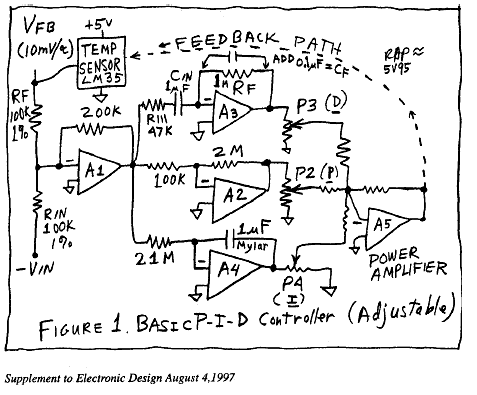
\includegraphics[scale = .5]{pease.png}
% \caption{Messy Hand Drawn circuit that is hard to follow.}
% \label{fig:MessyCircuit}
% \end{figure}

% \noindent
% Much like the equations, figures need to have numbering so that you can reference them properly within the document. Cite your images whenever you add an image that was not created on your own.

% \subsubsection{\LaTeX \hspace{0ex} vs. Word/Docs}
% It is worth mentioning that one of the other awesome benefits with using LaTeX is that it will semi-automatically number your equations and figures for you. Word and Docs should be able to do this as well, but the process can become very tiring when you have many equations and figures within a document.

Character echoing through hardware UART was explored in \href{https://github.com/RU09342/lab-1-intro-to-git-c-and-msp430-boorsteid4}{Lab 1: Introduction to C, Git, and the MSP430}. The example code provided initialized proper registers to enable UART on a series of MSP430 devices. It would have been possible, using serial communication software, to send a string of characters to the microprocessor's UART module through a terminal window and receive an echoed-back string of characters in the terminal window. Unfortunately, the example code was flawed: no characters were returned from the microprocessor. However incorrect the code, it nonetheless served as a good starting point for implementing UART.\\

\noindent The steps for initializing UART are not much different than those for GPIO or timers. Like these, UART has its own interrupt vector registers and associated interrupt flags. Many product lines in the MSP430 family of devices have embedded in the hardware a Universal Serial Communication Interface (USCI), a UART module. USCI architecture is generally shared among the devices, however some contain an updated module, the Enhanced USCI (eUSCI).

\subsection{USCI and eUSCI Modules}
The eUSCI module is essentially the updated version of the USCI, and can be in the MSP430FR2311, FR5994, and FR6989 models.

\section{Evaluation and Results}
This is where you will want to layout the steps you took to simulate, test, and evaluate the circuits in the lab. It is \textbf{\underline{SUPER IMPORTANT}} that you begin talking like engineers in these reports. This means two major things. First, you need to utilize \textbf{quantitative} language over \textbf{qualitative} language. Saying things like ``it worked, or it made sound'' really mean nothing. What is ``worked'' or what is your definition of success? Without laying this out, you basically have no grounds for your report. Utilize numbers and measurements to give your statements support rather than just putting out empty claims.
\\
\\
\noindent
The second thing that is required of an engineer is the explanation and defense of their decisions. Anytime that you hit a point where you must decide what values, parts, or even layouts to use, you \textbf{MUST} give an explanation as to why. For example, in Lab 2 when you calculated the current limiting resistor, you noticed that the specific resistance value was not available as a common resistor value. You were faced with a decision. Do you place multiple resistors in series/parallel to achieve the exact resistance (good luck with that)? Do you round your number up/down to the next value of resistance? And most importantly, \textbf{WHY DID YOU PICK THAT CHOICE?} Although it may be the answer at the time, you should never say ``We picked it 'cause it was close and stuff''. Give me measurements, uncertainties, arguments as to why one decision is better than the other. For example, I can tell you right now that putting multiple resistors in series would be the worst decision from an accuracy standpoint (look at the effect of cascading errors).

\subsection{Measurement Uncertainty}
One aspect of PECA and really any field of engineering is how we approximate the real world. For example, our resistors in the lab have a $\pm5\%$ tolerance. So even though the resistor may have a nominal values of 1000$\Omega$, this really can vary between 950$\Omega$-1050$\Omega$. What impact does this have on your circuit? If this is part of your amplifier circuitry, how does it impact the gain? What about with volume control, can that amount of resistance change be noticed?
\\
\\
\noindent
Now you may be thinking, ``Great, so I can just measure this stuff on the multimeter, write down the values to the 10th place and everything is good''. But in reality, those meters and scopes have uncertainties of their own. While they can be extremely precise, you need to take quite a few precautions before you can get to that accuracy. Also, all components that you deal with are impacted by the temperature they are running at. 
\\
\\
\noindent
This is all meant to show you that your measurements really are meaningless unless you give the uncertainties and the conditions in which you measured the values. We are not asking you to measure everything with NIST level accuracy, but start making measurements on components and sources that you normally would trust. Measure resistors before using them in your circuits, measure your voltage sources (those displays lie), try to get as accurate as possible.

\subsection{Results vs. Discussions}
One of the most common issues I have seen in the past is the separation between the Results and the Discussion within a app note. Most students tend to mix these two portions of their reports into one big section. In an app note or a technical paper, you want to separate out your data (results) into one section and your discussions into another. This way, you can easily reference back to the results as well as it provides one place where a reader can see all of your data.

\section{Discussion/Conclusions}
Now you can explain what you found during your experimentation and attempt to explain why certain things happened. You should do this with as much explanation and rigor as you can. For example, in Lab 2, you attempted to drive the speaker without the Op Amp. What happened? More importantly, why did you not only get little to no volume, but also a very very small range of volume control? Cite some analysis you did in the previous sections. Basically, try to be inquisitive like the engineers you are learning to be. Instead of just rolling with the punches, question why the hell would we want to add a \$15 component to something that could easily be pennies in cost? What value does it add? What are each of the components doing?
\\
\\
\noindent
Make sure that you cover every point made in the lab procedure. Anytime you see a question asked, make sure you have the answer. It is up to you as the writer, however, to determine the best place to address that question. If it is an analysis question, it might be better suited for the Background section, where as measurements and results belong in the results section. Use your judgment and take 10 minutes (preferably a lot more) to look up example app notes and see how those writers compose their documents.
\\
\\
\noindent
Overall, keep this in mind when you are writing your reports. Imagine you are handing this App Note to a student next year that is in the same position you were right before starting the lab. They should be able to replicate exactly what you did as well as the results you obtained. The steps you lay out in the app note are the ones they will follow. If you were handed this app note, would you be bored out of your mind? Would it be hard to follow the flow of the experiment? Remember that the people grading these are people too and these reports can become very dry very quickly when you have to grade 30 of them. Don't make the document a joke, but give it some personality if you want.


\end{document}

